\subsubsection*{Analysis}
\begin{tabular}{@{}l l}
\textbf{Scope}:&The AuctionHouse\textsuperscript{TM} automated administration system\\
\textbf{Level}:&User goal\\
\textbf{Primary Actor}:&Auctioneer\\
\textbf{Stakeholders and Interests}:&\begin{tabular}[t]{@{}l}Auctioneer: Wants to remove items from the item list;
\\Owner: Does not want to display non-existent items to the viewers;
\\Viewer: Wants to see only existent items and (if applicable) their actual quantity.  \end{tabular}\\
\textbf{Preconditions}:&\begin{tabular}[t]{@{}l}Actor is identified and authenticated.\\Actor is authorized to access this use case.\end{tabular}\\
\textbf{Postconditions}:&\begin{tabular}[t]{@{}l}The item list has been updated and does not contain the removed item. \end{tabular}\\
\textbf{Special requirements}:&\begin{tabular}[t]{@{}l}The item should be identifiable (perhaps with an unique identification number).\end{tabular}\\
\textbf{Frequency of occurence}:&Very frequent after each auction (once per month), otherwise rarely to even none at all.\\
\end{tabular}\\\\
\textsl{Main Success Scenario}
\begin{enumerate}[noitemsep]
	\item The user enters the deletion mode for items.
	\item An empty \textit{selectedForDeletion} list is created.
	\item The system displays a filterable list of all items.
	\item The user filters the list using the following items characteristics:
	\begin{itemize}[noitemsep]
		\item The amount of the item available
		\item The type of item
		\item A description
		\item If the item possesses any antiquarian value
		\item A minimum price decided by the owner
		\item The date when brought in
		\item Name and address of the owner plus identification
		\item Planned auction date
		\item Distinguishing features
	\end{itemize}
	\item The user selects an item from the resultant filtered (shrinked) list.
	\item If the item is already in the \textit{selectedForDeletion} list remove it and jump to 9.
	\item The systems prompts the user whether the item is surely removed from the stockroom.
	\item If the user answers yes - add the item to the \textit{selectedForDeletion} list, otherwise do nothing.
	\item If the user wants to modify the \textit{selectedForDeletion} list, repeat steps 3-9.
	\item Remove all items in the \textit{selectedForDeletion} list from the full item list and display the number of overall deleted items.
\end{enumerate}

\textsl{System Sequence Diagram}\\\\
\begin{figure}[H]
	\centering
	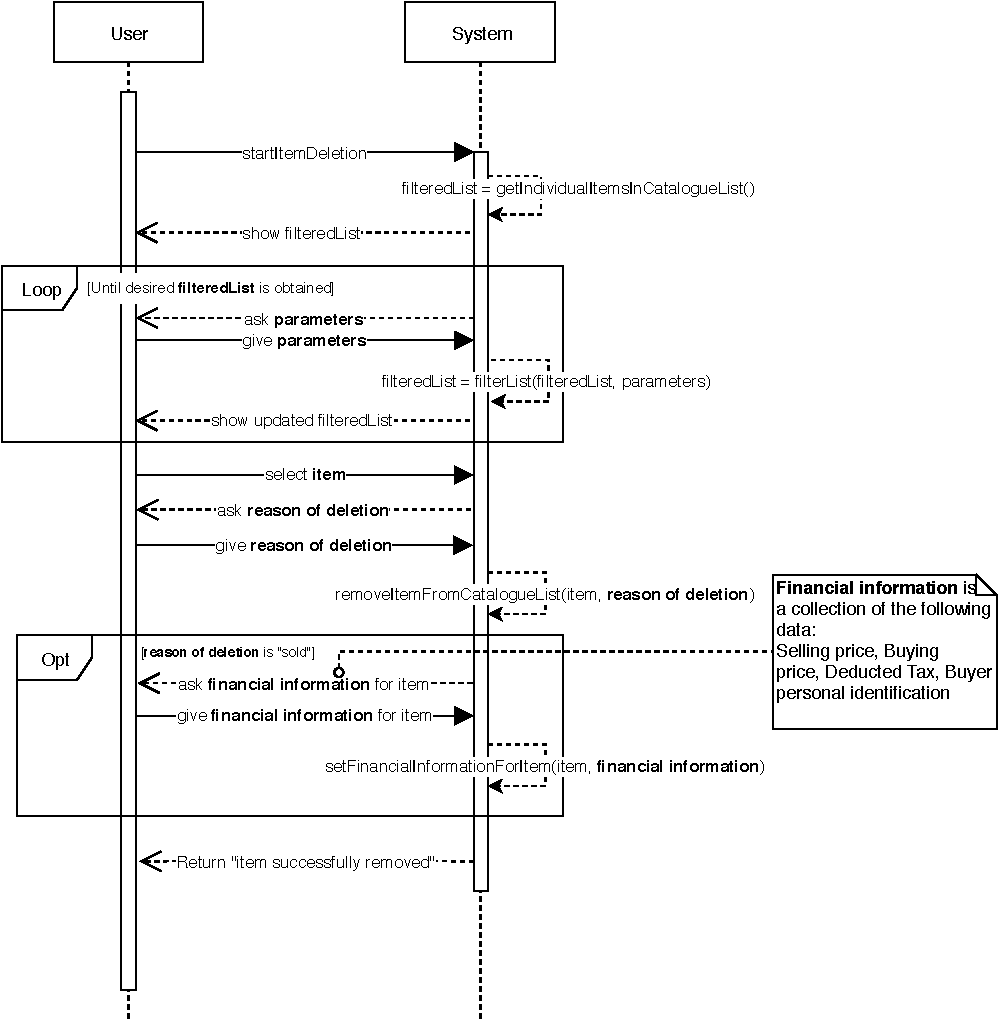
\includegraphics[scale=1]{uml/SD-bb-delete.pdf}
	\caption*{Interactions displayed in a System Sequence Diagram defined by the MSS and its extensions in blackbox format.}
\end{figure}